\documentclass[a4paper,11pt]{article}
\usepackage{style}

\begin{document}

\fiche{Synchronisation}

\titre{Condition de concurrence :} Deux processus manipulent des données partagées et le résultat final dépend de l'ordonnancement. \\
\titre{Section critique :} Partie du code dans laquelle deux proc ne doivent jamais se trouver en même temps. \\
\titre{4 règles d'or :} Pas en même temps en SC --- pas de supposition sur la vitesse, le nb de proc --- se dépêcher de quitter la SC --- jamais attendre indéfiniment l'accès à une SC.\\
\titre{Fork :} Crée new entrée ds table des proc. --- copie espace d'adressage  --- copie descripteurs de fichiers --- 0 = fils, pidfils = père --- père attend fils par wait ou waitpid.\\
\titre{Thread :} Nouvelle pile d'exécution. \\
\titre{Test and modify :} Ne marche pas \titre{Attente active :} Var verrou a val différente selon le proc. Pas bien \\
\titre{Producteur/Consommateur :} Situation classique (ex : spool d'impression) \\
\titre{Solution naïve :}
\begin{minipage}{0.45\linewidth}
Producteur :\\
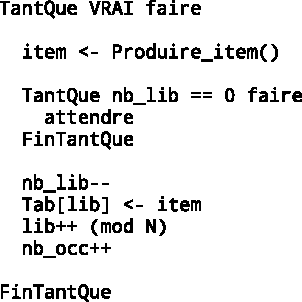
\includegraphics[width=0.6\linewidth]{fig12.pdf} 
\end{minipage}
\begin{minipage}{0.45\linewidth}
Consommateur :\\
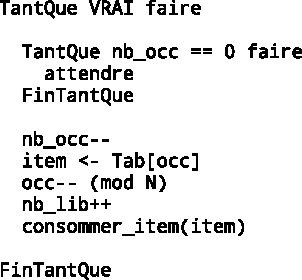
\includegraphics[width=0.6\linewidth]{fig13.pdf}
\end{minipage}\\
\titre{Sémaphore :} Un entier + fonctions POST(débloque ou incrémente) et WAIT(bloque ou décrémente) + file d'attente de threads bloqués. \\
\begin{minipage}{0.45\linewidth}
Producteur :\\
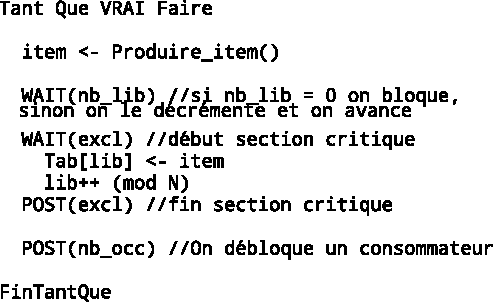
\includegraphics[width=0.9\linewidth]{fig17.pdf} 
\end{minipage}
\begin{minipage}{0.45\linewidth}
Consommateur :\\
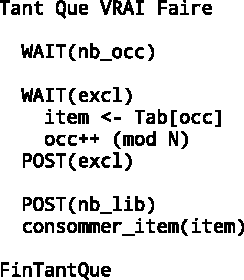
\includegraphics[width=0.4\linewidth]{fig18.pdf}
\end{minipage}\\
\titre{Sémaphore nommé :} Fichier virtuel utilisable par tous processus.\\
\titre{Sémaphore non nommé :} Variable du processus, utilisable que par les threads. \\
\begin{minipage}{0.3\linewidth}\titre{Mémoire partagée :} \\ 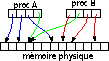
\includegraphics[width=\linewidth]{fig19.pdf}\end{minipage} \hspace{1cm}
\begin{minipage}{0.4\linewidth}\titre{Utilisation :} Fichier virtuel \begin{itemize} \item ouvre \item redimensionne(1x) \item projette \item détruit(1x) \end{itemize}\end{minipage}
\begin{minipage}{0.2\linewidth}\titre{Fork :} Le père et le fils partagent la mémoire \end{minipage}\\
\begin{minipage}{0.3\linewidth}\titre{Variables de conditions :} \\ 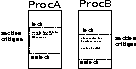
\includegraphics[width=\linewidth]{fig33.pdf}\end{minipage} \hspace{1cm}
\begin{minipage}{0.7\linewidth}\titre{Explication :} De manière atomique, on déverrouille le mutex et on passe en attente de la condition. Lorsque la condition est remplie, on passe de façon atomique à mutex verrouillé. \end{minipage}\\
\titre{Barrière :} barrier\_wait bloque le thread jusqu'à ce que suffisament de processus aient atteint barrier\_wait \\
\titre{Tubes nommés :} mkfifo \titre{Non nommés :} symbole pipe entre 2 proc ou pipe(df[2]) \\
\titre{Resource :} Objet physique ou virtuel pouvant être alloué à un seul processus à la fois.\\
\titre{Resources retirables :} Peut être retirée au processus, utilisée par un autre, puis rendue au 1er sans compromettre son exécution (ex. CPU, RAM). \\
\titre{Resources non retirables :} Ne peut être retirée au processus que lorsqu'il en aura décidé. \\

\titre{Famine :} Situation où un processus demande l'accès à une ressource mais ne l'obtient jamais car elle est toujours attribuée à d'autres processus.\\
\titre{Solution :} Le principe FIFO permet d'éviter la famine mais n'est pas toujours souhaitable. \\
\titre{Interblocage :} Situation où un ensemble de processus attendent un événement que seul un des processus de l'ensemble peut provoquer.\\
\begin{minipage}{0.5\linewidth} \titre{Modèle de Holt :} \\Carré = ressource, Rond = processus
\end{minipage} \hspace{1cm}
\begin{minipage}{0.15\linewidth}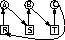
\includegraphics[width=\linewidth]{fig38.pdf} \\ \end{minipage}\\
\begin{minipage}{0.7\linewidth}\titre{Etats surs :}  On appelle état sûr un état à partir duquel on peut exécuter tous les processus un après l'autre dans un certain ordre sans qu'aucun ne soit bloqué. Un interblocage survient toujours à partir d'un état non sûr. \\ Pour déterminer les états sûrs, il faut connaitre à l'avance le code que vont exécuter les programmes. 
\end{minipage} \hspace{1cm}
\begin{minipage}{0.2\linewidth}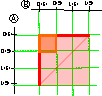
\includegraphics[width=\linewidth]{fig39.pdf} \\ \end{minipage}\\
\titre{Stratégies possibles pour les interblocages :} Ignorer --- Détecter et remédier (Holt) --- Eviter (états sûrs) --- Contraintes (pas d'exclusion mutuelle, ordonner les ressources).\\

\titre{Fork : } pid\_t fork(void) \\ pid\_t waitpid(pid\_t pid, int* status, int options) --- pid\_t wait(int *status) \\
\titre{Threads : } int pthread\_create(pthread\_t * thread, NULL, (void*(*)(void *))f, (void*)data) \\ pthread\_exit(void* retval) --- pthread\_join(pthread\_t th, void **thread\_return)\\
\titre{Sémaphores :} int sem\_post(sem\_t *sem) --- int sem\_wait(sem\_t *sem) \\ int sem\_trywait(sem\_t *sem) --- int sem\_getvalue(sem\_t *sem, int *sval)\\
\titre{Non nommés :} int sem\_init(sem\_t *sem, int pshared(0=threads seulement), int value) \\ sem\_destroy(sem\_t *sem)\\
\titre{Nommés :} sem\_t *sem\_open(const char *name, int oflag(O\_CREAT|O\_EXCL), mode\_t mode(S\_IRWXU), int value) --- sem\_t *sem\_open(const char *name, int oflag(O\_RDWR)) \\ sem\_close(sem\_t *sem) --- sem\_unlink(const char *name).\\
\titre{Mutex :} pthread\_mutex\_init(pthread\_mutex\_t *mutex) \\ pthread\_mutex\_lock(pthread\_mutex\_t *mutex) --- pthread\_mutex\_unlock(pthread\_mutex\_t *mutex) \\ pthread\_mutex\_trylock(pthread\_mutex\_t *mutex) --- pthread\_mutex\_destroy(pthread\_mutex\_t *mutex)\\
\titre{Mémoire partagée :} int shm\_open(const char *nom, int oflag, mode\_t mode) \\ ftruncate(int df, off\_t length) \\ void *mmap(void *addr, size\_t length, int prot(PROT\_READ|PROT\_WRITE), MAP\_SHARED, int df, off\_t offset) \\ int munmap(void *addr, size\_t length) --- int shm\_unlink(const char *nom)\\
\titre{Variables de condition :} int pthread\_cond\_init(pthread\_cond\_t *cond, NULL) \\ int pthread\_cond\_signal(pthread\_cond\_t *cond) \\ int pthread\_cond\_broadcast(pthread\_cond\_t *cond) \\ int pthread\_cond\_wait(pthread\_cond\_t *cond, pthread\_mutex\_t *mutex) \\ int pthread\_cond\_destroy(pthread\_condèt *cond)\\
\titre{Barrière :} int pthread\_barrier\_init(pthread\_barrier\_t *barrier, NULL, count) \\ int pthread\_barrier\_wait(pthread\_barrier\_t *barrier) \\ int pthread\_barrier\_destroy(pthread\_barrier\_t *barrier) \\
\titre{Tube :} ssize\_t read(int df, void *buf, size\_t count) \\ ssize\_t write(int fd, void *buf, size\_t count)\\
\titre{Nommé :} int mkfifo(const char *pathname, mode\_t mode) \titre{Non nommé :} int pipa(int pipefd[2])

\end{document}
